% Insert inside the report's Experimental Results section.
% Replace the existing E1 subsection rather than appending a second copy.
% Required packages: graphicx, booktabs.
% Companion appendix: e1_story_appendix.tex (insert after \appendix).

\subsection{E1: Baseline Performance of a FIFO ROS2--REST Gateway under Increasing Traffic Load}
\label{sec:e1story}

\subsubsection{Experimental Objective and Procedure}

E1 investigated how increasing mixed traffic affects a baseline
ROS2-to-REST gateway. The experiment first assessed whether completed
throughput kept pace with offered traffic, then examined queue growth,
message delay, deadline failures and resource use.

The baseline used one gateway, one REST server, a persistent HTTP/1.1
connection and one outstanding request at a time. A FIFO queue held up
to 1,000 waiting messages, excluding the request in service. Newly
arriving messages were discarded when the queue was full. Application
retries, compression and injected network impairments were disabled.
The generator, gateway and server ran on the same Ubuntu 22.04 WSL2
host, with HTTP traffic using loopback.

\begin{table}[htbp]
    \centering
    \caption{Base traffic per robot-equivalent. Payload sizes exclude
    JSON metadata and protocol headers. Deadlines are illustrative
    project targets, fixed before the sweep.}
    \label{tab:e1story-traffic}
    \small
    \setlength{\tabcolsep}{3pt}
    \begin{tabular}{lrrr}
        \toprule
        Class & Rate (Hz) & Payload (B) & Deadline (ms) \\
        \midrule
        Command  & 2  & 100    & 100 \\
        Status   & 5  & 100    & 200 \\
        Odometry & 20 & 250    & 100 \\
        Sensor   & 5  & 20,000 & 1,000 \\
        \bottomrule
    \end{tabular}
\end{table}

Table~\ref{tab:e1story-traffic} defines a total of 32 messages/s per
robot-equivalent. The tested loads were
$N\in\{1,2,4,8,16,32,64\}$, giving nominal totals of $32N$ messages/s.
One ROS2 robot node was used at $N=1$ and two at all other loads.
For $N\geq2$, each node published at $N/2$ times the base rates while
payload sizes remained fixed. Thus, these conditions represent
robot-equivalent traffic volume rather than $N$ independent robot nodes
or HTTP clients.

Each robot/class stream had a seeded initial offset and then published
periodically. The source published whichever stream was due next,
independently of HTTP response completion. The gateway served admitted
messages in queue-arrival order without class priority, waiting for one
response before sending the next request.

Every load was repeated three times, producing 21 runs in a seeded
shuffled order. Each run used a five-second warm-up, a 60-second
measurement window and up to 15 seconds to drain outstanding work.
Repetitions used different reproducible initial publishing phases.
Every generated message had a unique identifier, with timestamps
recorded for each stage it reached.

Latency was measured from generation until the gateway received and
parsed the response. It therefore includes ROS2 delivery, queue waiting,
request serialisation and the HTTP exchange. Latency statistics use
successful messages generated during measurement, including responses
received during the bounded drain. Deadline-failure ratios include all
messages generated during measurement, including unsuccessful messages.
Throughput and goodput instead count completions within the measurement
window; these populations differ at the boundaries.

For each load-sweep plot, a statistic was calculated separately for
each run. Points show the mean of the three run-level statistics and
error bars show their minimum and maximum, not confidence intervals.
In particular, the latency points average three run-level p95 values
rather than calculating a percentile from pooled messages.

\paragraph{Packet-level validation.}
A separate five-minute, two-robot validation run supplied packet
evidence for the baseline configuration. Scripted capture analysis
identified one initial TCP connection attempt and 19,520 HTTP/1.1 POST
requests with matching 200 responses, including warm-up. These counts
matched the server log; the 300-second measurement cohort alone
contained 19,200 messages. Captured IPv4 traffic exceeded configured
application payload bytes by 27.72\%, including JSON metadata, HTTP
headers and responses, and TCP/IP headers. This is loopback byte
accounting, not physical Ethernet utilisation. The capture includes
the initial handshake but omits the final teardown.
% Add a Wireshark screenshot only after inspecting the existing capture.
% Do not describe this capture as covering the entire 21-run load sweep.

Having established the baseline configuration, the first question is
whether the gateway completes traffic as quickly as it is offered.

\subsubsection{Throughput under Increasing Load}

Completed throughput was calculated by dividing the number of
successful responses completed inside each measurement window by
60 seconds. Figure~\ref{fig:e1story-throughput} compares this rate with
the total generation rate across all four classes. The dashed line
marks completion rate equal to offered rate.

\begin{figure}[htbp]
    \centering
    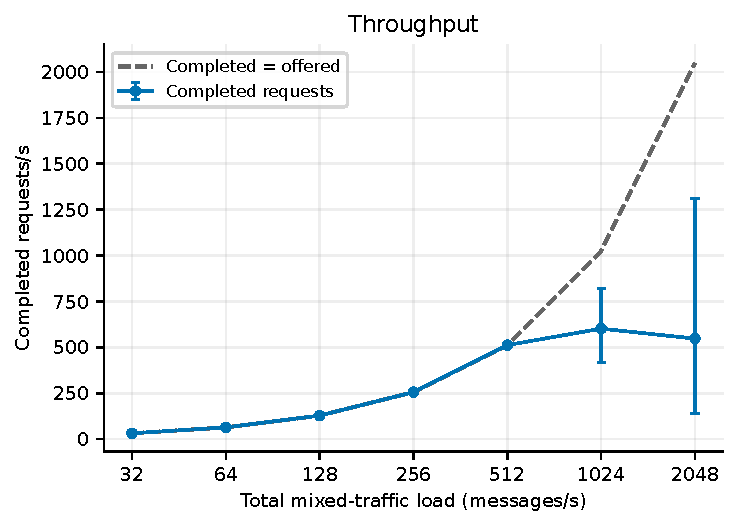
\includegraphics[width=\columnwidth]{figures/fig4_throughput.pdf}
    \caption{Completed throughput versus total mixed-traffic load.
    Points are means of three runs; error bars show minimum--maximum.
    The dashed line represents completion rate equal to offered rate.}
    \label{fig:e1story-throughput}
\end{figure}

Mean completion rate closely followed offered traffic through
16 equivalents. At a nominal 512 messages/s, completed throughput
averaged 512.1 requests/s; the small excess reflects measurement-window
boundary effects. At 32 and 64 equivalents, completion rates averaged
601.8 and 547.5 requests/s despite nominal offered rates of 1,024 and
2,048 messages/s. The measured path therefore could not keep up under
those higher-load conditions. Large error bars at high load prevent
interpreting the mean curve as a precise, stable capacity boundary.
Payload goodput provides a complementary view in
Figure~\ref{fig:e1story-goodput}.

This throughput shortfall raises the question of what happens to
messages awaiting transmission.

\subsubsection{Queue Accumulation and Overflow}

Waiting-queue length was reconstructed from timestamped queue events.
Mean occupancy was obtained by weighting each queue length by the time
for which it persisted, integrating over the measurement window and
dividing by its duration. The request already in service was excluded.
Figure~\ref{fig:e1story-queue} averages these run-level time averages.

\begin{figure}[htbp]
    \centering
    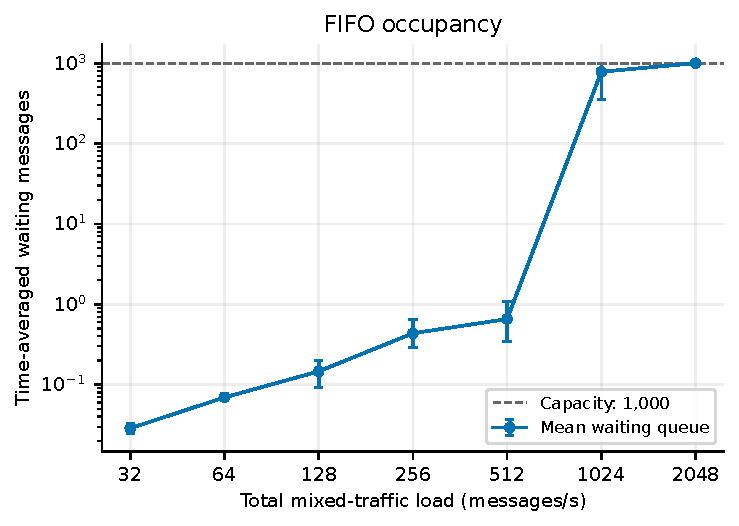
\includegraphics[width=\columnwidth]{figures/fig3_queue.pdf}
    \caption{Time-averaged FIFO occupancy versus total mixed-traffic
    load. The dashed line marks the capacity of 1,000 waiting messages.
    Points are means of three runs; error bars show minimum--maximum.}
    \label{fig:e1story-queue}
\end{figure}

Mean occupancy increased from 0.65 messages at 16 equivalents to
782.67 at 32 equivalents and 999.69 at 64 equivalents. The highest-load
queue therefore remained almost full. Once a bounded FIFO fills,
additional arrivals may be dropped rather than increasing its length.
Combining counts across repetitions, 40.68\% and 73.27\% of generated
messages were dropped at admission at 32 and 64 equivalents,
respectively. Figures~\ref{fig:e1story-drops}
and~\ref{fig:e1story-trace} provide supporting drop statistics and
selected queue traces.

Queue accumulation affects both the number of messages delivered and
the delay experienced by messages that do complete.

\subsubsection{Consequences for Latency and Deadlines}

Generation-to-response delays were grouped by traffic class, and p95
latency was calculated separately for each run. The points in
Figure~\ref{fig:e1story-latency} average those three p95 values.
Each coloured curve represents one class under the same mixed
workload: at $N=1$, for example, odometry contributes 20 messages/s
within a total of 32 messages/s.

\begin{figure}[htbp]
    \centering
    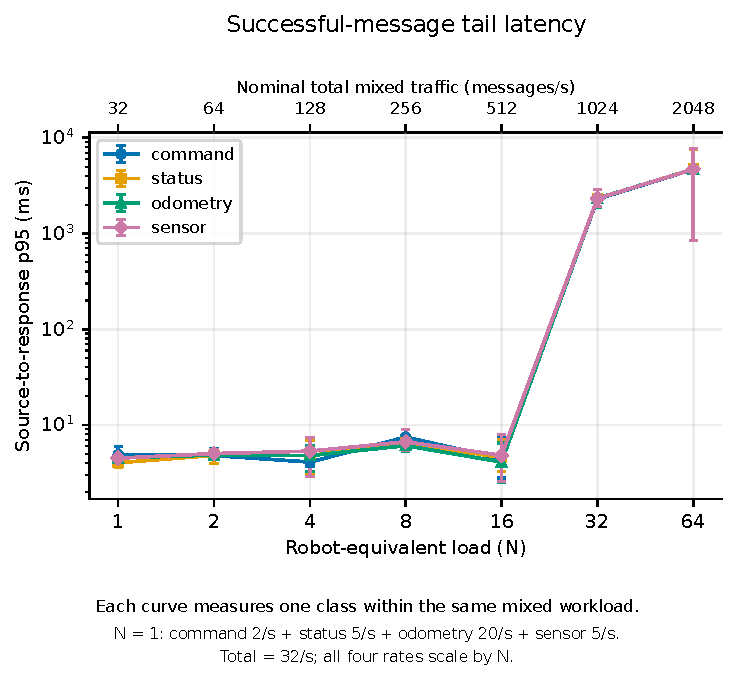
\includegraphics[width=\columnwidth]{figures/fig1_latency.pdf}
    \caption{Per-class successful-message p95 source-to-response latency.
    The bottom axis is robot-equivalent load $N$; the top axis is total
    nominal mixed traffic, $32N$ messages/s. Points average three
    run-level p95 values; error bars show minimum--maximum.}
    \label{fig:e1story-latency}
\end{figure}

Mean run-level p95 latency remained below 8 ms for every class across
the 1--16-equivalent conditions. At 32 equivalents, class-specific
means rose to approximately 2.3 s, reaching approximately 4.7 s at
64 equivalents. Odometry p95, for example, increased from 4.10 ms at
16 equivalents to 4,691.65 ms at 64 equivalents. The increase coincides
with queue accumulation. Similar class delays under overload are
consistent with a shared FIFO that provides no class priority; they
do not establish identical service costs for the different payloads.

Latency alone excludes messages that never complete. To assess the
whole generated workload, each message was also compared with its
class's fixed deadline. A failure was either a late response or an
unsuccessful message, including a FIFO drop. For each class and run,
the failure count was divided by all messages generated during
measurement. Figure~\ref{fig:e1story-deadlines} averages the resulting
run-level percentages.

\begin{figure}[htbp]
    \centering
    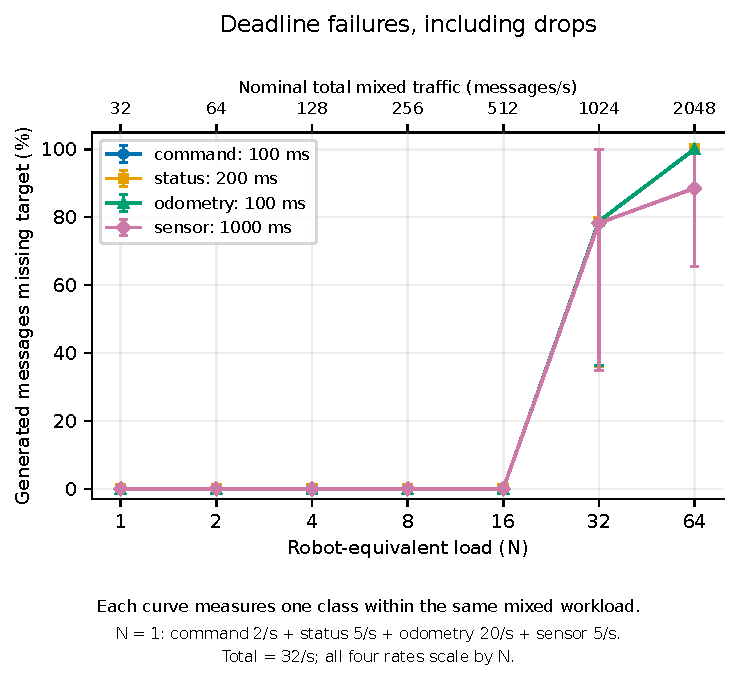
\includegraphics[width=\columnwidth]{figures/fig2_deadlines.pdf}
    \caption{Deadline failures, including late and unsuccessful
    messages. Targets are command 100 ms, status 200 ms, odometry
    100 ms and sensor 1,000 ms. The axes describe the same mixed
    workload as Figure~\ref{fig:e1story-latency}. Points are means of
    three runs; error bars show minimum--maximum.}
    \label{fig:e1story-deadlines}
\end{figure}

No deadline failures were observed through 16 equivalents. At
32 equivalents, approximately 78\% of each class failed its target.
At 64 equivalents, every command, status and odometry message failed,
while sensor failures averaged approximately 88.5\%. The smaller
sensor failure percentage does not demonstrate preferential service:
sensor messages had a looser deadline, and class delivery outcomes
also differed. These findings motivate a later controlled comparison
of FIFO and priority scheduling.

The results establish overload and its consequences. Resource
measurements next help identify which parts of the implementation
warrant investigation.

\subsubsection{Investigating the Bottleneck}

Cumulative process CPU counters were sampled every 0.2 seconds and
interpolated at the measurement boundaries. CPU-time increments were
divided by the window duration and expressed as percentages. Here,
100\% represents one logical CPU, so a multithreaded process can
exceed 100\%.

\begin{figure}[htbp]
    \centering
    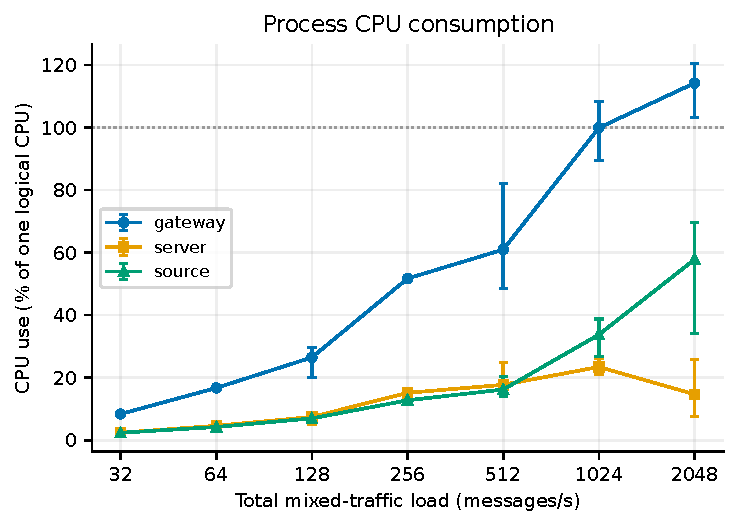
\includegraphics[width=\columnwidth]{figures/fig5_cpu.pdf}
    \caption{Process CPU consumption versus total mixed-traffic load,
    normalised to one logical CPU. Points are means of three runs;
    error bars show minimum--maximum.}
    \label{fig:e1story-cpu}
\end{figure}

At 64 equivalents, gateway CPU consumption averaged 114.2\% of one
logical CPU, compared with 57.8\% for the source and 14.7\% for the
server. Figure~\ref{fig:e1story-cpu} therefore directs attention towards
the gateway/client processing path. It does not demonstrate exhaustion
of the whole machine or establish the server's maximum capacity.

CPU consumption was complemented by occupied wall time. Sender
activity was measured from dequeue until response completion. Server
activity was measured from POST-handler entry to completion of the
response write, including body-read waiting but excluding header
parsing and idle time before the handler started. Intervals were
clipped to the measurement window and their total duration divided
by the window length. These measures include waiting as well as
execution, so they differ from CPU percentages.

\begin{figure}[htbp]
    \centering
    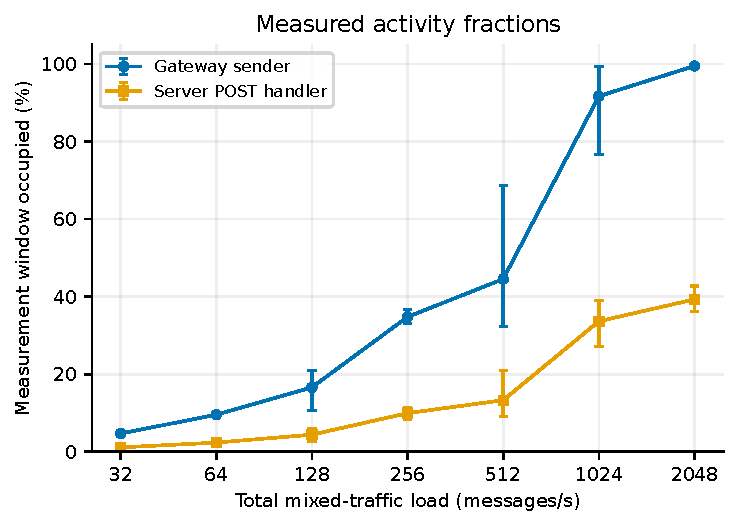
\includegraphics[width=\columnwidth]{figures/fig6_busy_time.pdf}
    \caption{Sender and server POST-handler occupied fractions.
    Timing boundaries are defined in the text. Points are means of
    three runs; error bars show minimum--maximum. Occupied time is
    distinct from CPU consumption.}
    \label{fig:e1story-busy}
\end{figure}

At 64 equivalents, the sender was occupied for 99.5\% of the window,
compared with 39.3\% for the server handler
(Figure~\ref{fig:e1story-busy}). For successful messages, averaging
the per-run mean delays gave 4,175.88 ms of queue waiting versus
3.98 ms from dequeue to response completion, including serialisation,
the HTTP exchange and response parsing. Queue waiting dominated
completed-message delay. Together, these observations implicate the
serial gateway/client path without establishing server or physical-link
saturation. Adding server workers alone cannot be assumed to improve
a gateway restricted to one outstanding request.

\subsubsection{Repeat Variability and Experimental Limitations}

The overload outcome was consistent at 32 and 64 equivalents, but its
severity varied substantially. At 64 equivalents, completed throughput
ranged from 139.12 to 1,309.05 requests/s across repetitions, while
run-level p95 latency across successful traffic ranged from 851.40 to
7,649.29 ms. All runs were retained. These observations limit claims
about a single stable service-capacity threshold.

Figures~\ref{fig:e1story-within-cpu}
and~\ref{fig:e1story-within-queue} also show a change within the
32-equivalent, repeat-1 run. Repeat numbers identify seeded repetitions,
not chronological order. CPU consumption and queue occupancy changed
despite fixed configured publishing rates, but the measurements do not
establish the cause.

The shared-host loopback environment and rate-scaled synthetic traffic
limit generalisation to independent physical robots or a physical
network. Periodic arrivals and heterogeneous messages also do not
establish the assumptions of an M/M/1 model. Subsequent comparisons
should recheck the reference condition and account for execution
variability before attributing changes to a protocol or scheduling policy.

\subsubsection{Baseline Findings and Selection of Test Loads}

The highest tested load without FIFO drops or deadline failures in any
repetition was 16 robot-equivalents. Every 32- and 64-equivalent run
overflowed, making 64 equivalents useful as an overload stress
configuration. E1 therefore provides candidate reference and stress
conditions for later experiments, while showing that the FIFO baseline
does not protect timely communication under overload.

Table~\ref{tab:e1story-summary} retains the overall latency and payload
goodput measurements alongside the figures. Latency percentiles are
computed across successful traffic within each run before averaging
across repetitions.

\begin{table*}[t]
    \centering
    \caption{E1 summary. Values are means of three run-level statistics,
    except nominal load and pooled FIFO drop percentages. Latency
    includes successful messages only; goodput counts application
    payload bytes. Large repeat variability is discussed in the text.}
    \label{tab:e1story-summary}
    \small
    \setlength{\tabcolsep}{4pt}
    \begin{tabular}{rrrrrrrrr}
        \toprule
        Equiv. & Nominal & Completed & p50 & p95 & p99 & Mean & Goodput & FIFO \\
        & (msg/s) & (req/s) & (ms) & (ms) & (ms) & queue & (Mb/s) & drop (\%) \\
        \midrule
        1  & 32   & 32.0  & 3.56    & 4.54    & 5.45    & 0.03   & 0.85  & 0.00 \\
        2  & 64   & 64.0  & 3.63    & 4.99    & 6.05    & 0.07   & 1.69  & 0.00 \\
        4  & 128  & 128.0 & 3.30    & 4.99    & 5.87    & 0.15   & 3.38  & 0.00 \\
        8  & 256  & 256.0 & 3.70    & 6.37    & 7.95    & 0.44   & 6.76  & 0.00 \\
        16 & 512  & 512.1 & 2.58    & 4.42    & 8.54    & 0.65   & 13.53 & 0.00 \\
        32 & 1024 & 601.8 & 1361.06 & 2329.82 & 2453.45 & 782.67 & 11.99 & 40.68 \\
        64 & 2048 & 547.5 & 4363.20 & 4689.89 & 4811.69 & 999.69 & 7.62  & 73.27 \\
        \bottomrule
    \end{tabular}
\end{table*}
